% Options for packages loaded elsewhere
\PassOptionsToPackage{unicode}{hyperref}
\PassOptionsToPackage{hyphens}{url}
%
\documentclass[
  11pt,
]{article}
\usepackage{amsmath,amssymb}
\usepackage{iftex}
\ifPDFTeX
  \usepackage[T1]{fontenc}
  \usepackage[utf8]{inputenc}
  \usepackage{textcomp} % provide euro and other symbols
\else % if luatex or xetex
  \usepackage{unicode-math} % this also loads fontspec
  \defaultfontfeatures{Scale=MatchLowercase}
  \defaultfontfeatures[\rmfamily]{Ligatures=TeX,Scale=1}
\fi
\usepackage{lmodern}
\ifPDFTeX\else
  % xetex/luatex font selection
  \setmainfont[]{Times New Roman}
\fi
% Use upquote if available, for straight quotes in verbatim environments
\IfFileExists{upquote.sty}{\usepackage{upquote}}{}
\IfFileExists{microtype.sty}{% use microtype if available
  \usepackage[]{microtype}
  \UseMicrotypeSet[protrusion]{basicmath} % disable protrusion for tt fonts
}{}
\makeatletter
\@ifundefined{KOMAClassName}{% if non-KOMA class
  \IfFileExists{parskip.sty}{%
    \usepackage{parskip}
  }{% else
    \setlength{\parindent}{0pt}
    \setlength{\parskip}{6pt plus 2pt minus 1pt}}
}{% if KOMA class
  \KOMAoptions{parskip=half}}
\makeatother
\usepackage{xcolor}
\usepackage[margin=1in]{geometry}
\usepackage{graphicx}
\makeatletter
\def\maxwidth{\ifdim\Gin@nat@width>\linewidth\linewidth\else\Gin@nat@width\fi}
\def\maxheight{\ifdim\Gin@nat@height>\textheight\textheight\else\Gin@nat@height\fi}
\makeatother
% Scale images if necessary, so that they will not overflow the page
% margins by default, and it is still possible to overwrite the defaults
% using explicit options in \includegraphics[width, height, ...]{}
\setkeys{Gin}{width=\maxwidth,height=\maxheight,keepaspectratio}
% Set default figure placement to htbp
\makeatletter
\def\fps@figure{htbp}
\makeatother
\setlength{\emergencystretch}{3em} % prevent overfull lines
\providecommand{\tightlist}{%
  \setlength{\itemsep}{0pt}\setlength{\parskip}{0pt}}
\setcounter{secnumdepth}{-\maxdimen} % remove section numbering
\usepackage{setspace}
\doublespacing
\ifLuaTeX
  \usepackage{selnolig}  % disable illegal ligatures
\fi
\IfFileExists{bookmark.sty}{\usepackage{bookmark}}{\usepackage{hyperref}}
\IfFileExists{xurl.sty}{\usepackage{xurl}}{} % add URL line breaks if available
\urlstyle{same}
\hypersetup{
  pdftitle={Your Title Here},
  pdfauthor={Your Name},
  hidelinks,
  pdfcreator={LaTeX via pandoc}}

\title{Your Title Here}
\author{Your Name}
\date{2024-08-14}

\begin{document}
\maketitle

\hypertarget{introduction}{%
\section{Introduction}\label{introduction}}

This is the introduction section where you can provide an overview of
your analysis.

\hypertarget{graph-4.1}{%
\subsection{Graph 4.1}\label{graph-4.1}}

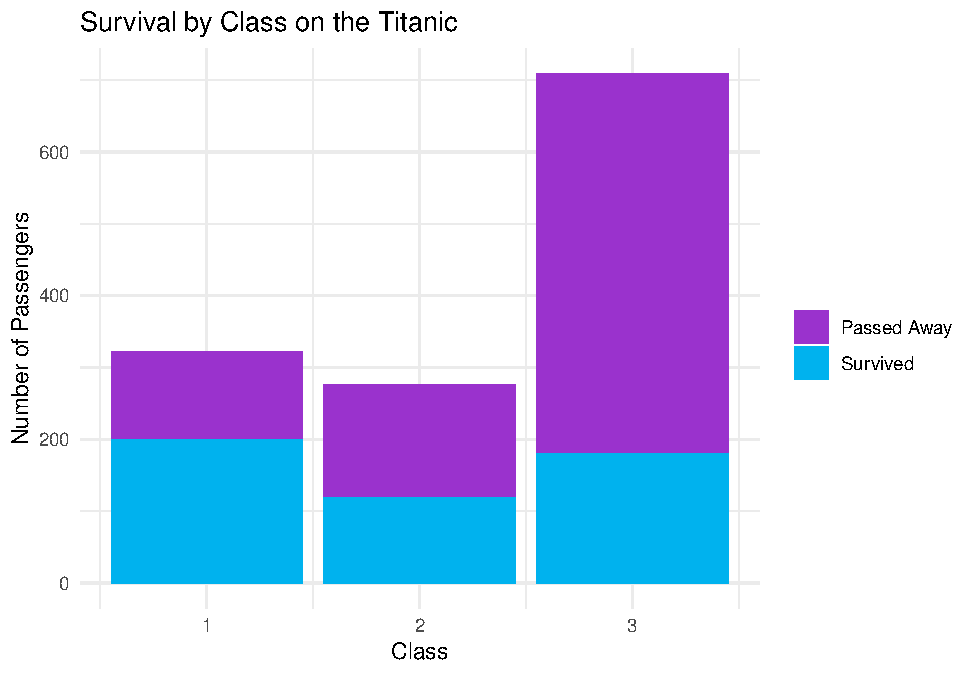
\includegraphics{README_files/figure-latex/unnamed-chunk-2-1.pdf}

\hypertarget{graph-4.2}{%
\subsection{Graph 4.2}\label{graph-4.2}}

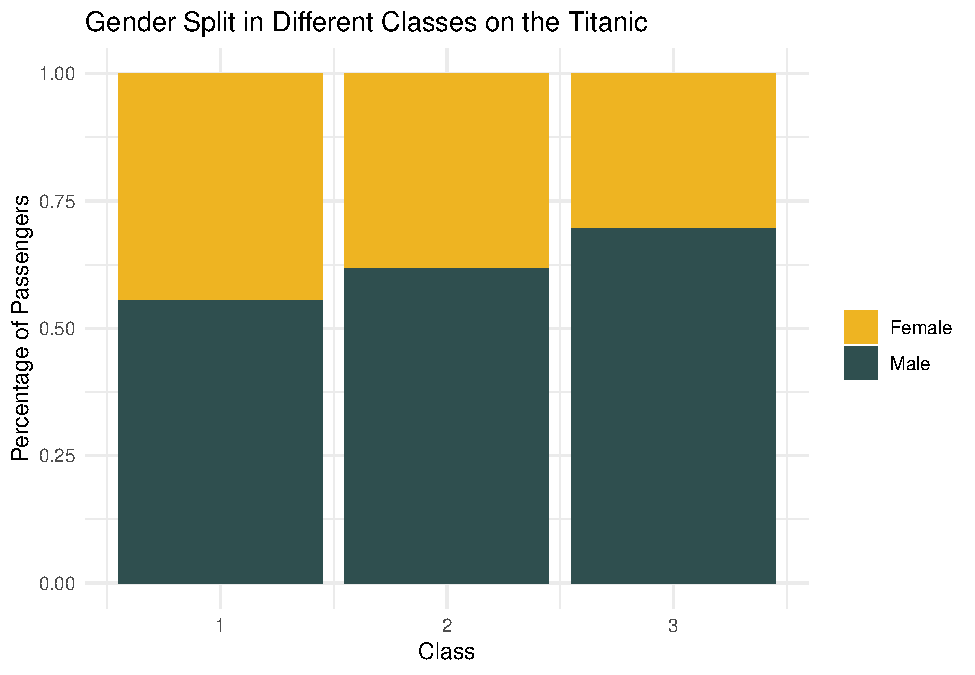
\includegraphics{README_files/figure-latex/unnamed-chunk-3-1.pdf}

\hypertarget{graph-4.3}{%
\subsection{Graph 4.3}\label{graph-4.3}}

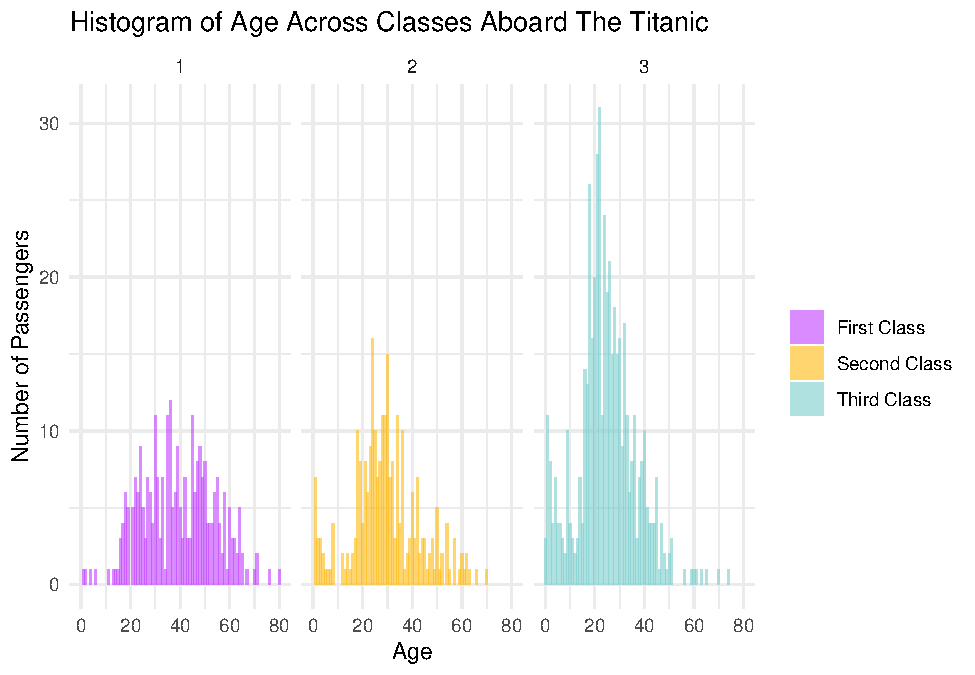
\includegraphics{README_files/figure-latex/unnamed-chunk-4-1.pdf}

\hypertarget{graph-4.4}{%
\subsection{Graph 4.4}\label{graph-4.4}}

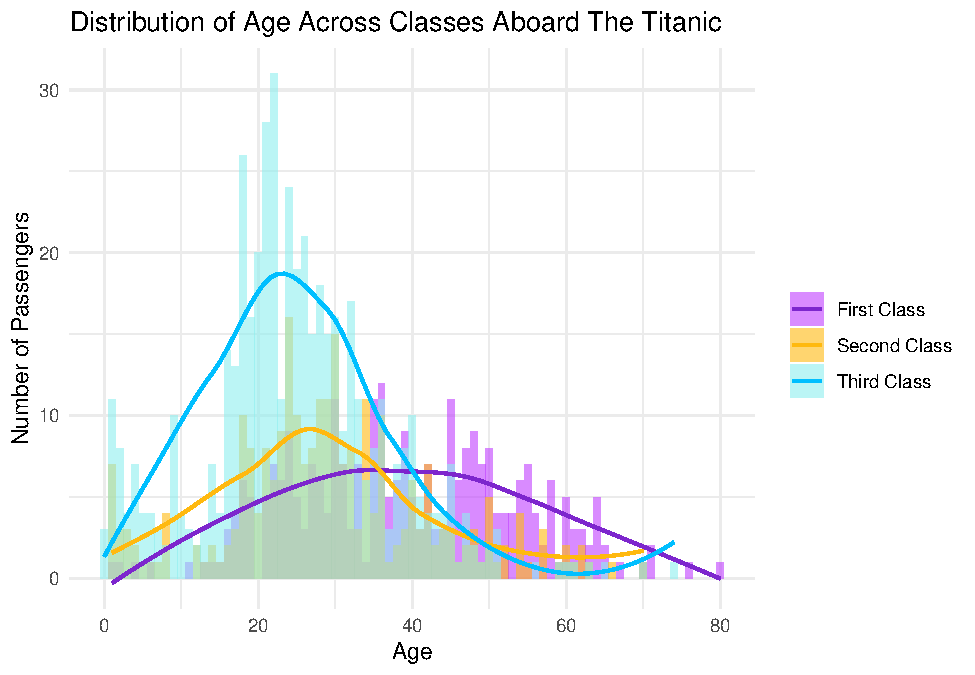
\includegraphics{README_files/figure-latex/unnamed-chunk-5-1.pdf}

\hypertarget{graph-4.5}{%
\subsection{Graph 4.5}\label{graph-4.5}}

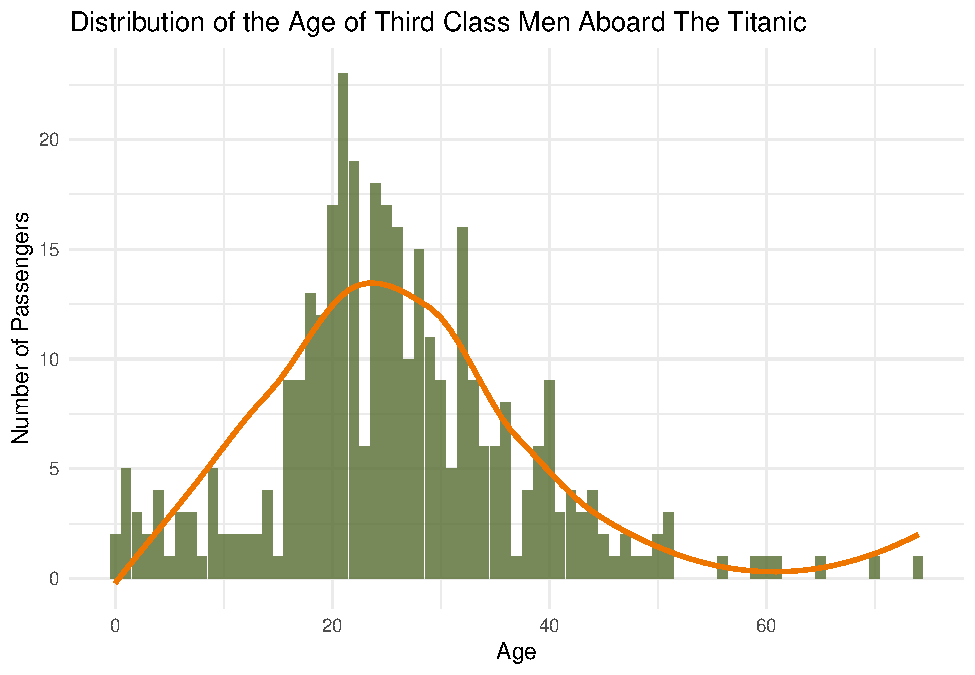
\includegraphics{README_files/figure-latex/unnamed-chunk-6-1.pdf}

\hypertarget{graph-4.6}{%
\subsection{Graph 4.6}\label{graph-4.6}}

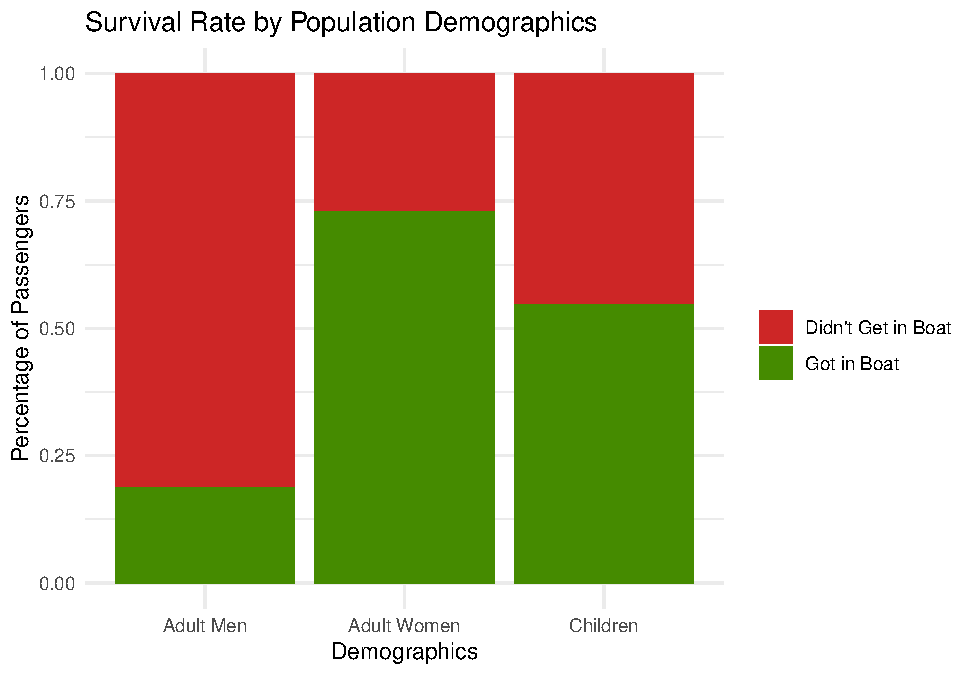
\includegraphics{README_files/figure-latex/unnamed-chunk-7-1.pdf}

\end{document}
